\documentclass[12pt,a4paper,oneside,open=right,%
bibliography=totoc,BCOR=10mm]{scrreprt} % Schriftgröße, Seitenformat, Zweiseitig für Seitenränder, Bindcorrection
\usepackage{ifpdf}
\ifpdf
  \input{glyphtounicode.tex}    %Part of modern distribution
  \input{glyphtounicode-cmr.tex}     %Additionnal glyph: You must grab it from pdfx package
  \pdfgentounicode=1
  \pdfinterwordspaceon
  \usepackage[a-2u,pdf17]{pdfx}
  \pdfomitcharset 1
\else  %Place here the settings for other compilator
\fi
%Encoding + cmap (to get proper UTF8 mapping)
%------------------------------------------------------
\usepackage{cmap}
\usepackage[utf8]{inputenc} % Richtiges anzeigen von Umlauten und quasi allen anderen Schriftzeichen
\usepackage[T1]{fontenc} % Wichtig für alles was mehr als ASCII verwendet
\usepackage{csquotes} % Schöne Anführungsstriche mit \enquote{Text}
\usepackage{amsmath} % Bessere und schönere mathematische Formeln
\usepackage{mathtools} % Noch schönerere mathematische Formeln
\usepackage{amstext} % \text{} Macro in mathematischen Formeln
\usepackage{amsfonts} % Erweiterte Zeichensätze für mathematische Formeln
\usepackage{amssymb} % Spezielle mathematische Symbole.
\usepackage{booktabs}
%Correct UTF8 mapping for ams fonts
\ifdefined\pdffontattr% \ifdefined is part of the e-TeX extension, which is part of any modern LaTeX compiler.
    \immediate\pdfobj stream file {umsa.cmap}
    {\usefont{U}{msa}{m}{n}\pdffontattr\font{/ToUnicode \the\pdflastobj\space 0 R}}
    \immediate\pdfobj stream file {umsb.cmap}
    {\usefont{U}{msb}{m}{n}\pdffontattr\font{/ToUnicode \the\pdflastobj\space 0 R}}
\fi
\usepackage{array} % Matrizen in mathematischen Formeln
\usepackage{textcomp} % Für textmu und textohm etc. um im Fließtext keine Mathematik 
\usepackage{textalpha} % Damit können griechische Zeichen direkt im Text verwendet werden (siehe zeichen.txt)
\usepackage{paralist} % Für compactitem und compactenum
\usepackage{xstring} % Für IF in Titelseite

\usepackage[version=3]{mhchem} % Für Chemische Formeln
\usepackage{braket} % Für das quantenmechanische Bra-Ket

\usepackage{geometry} % Seitenränder und Seiteneigenschaften setzen
%\usepackage[showframe]{geometry} % Anzeigen der Seitenränder, nützlich für debugging. http://ctan.org/pkg/geometry

\usepackage[bottom]{footmisc} % Zwingt Fußnoten an das Ende der Seite
\usepackage[pdftex]{hyperref} % Links richtig anzeigen. Sowohl innerhalb des Dokuments (Fußzeilen, Formeln), als auch ins Internet

\usepackage[ % Biblatex für die Zitate und Referenzen
	backend=biber,
	hyperref=true
		]{biblatex}

\usepackage{xkeyval} % Erlaubt "Variablen" zu definieren, wird für Titelseite gebraucht
\usepackage{graphicx} % Wichtig für das Einbinden von Grafiken
\usepackage{caption}
\usepackage{subcaption} % Einbinden von mehreren Grafiken in einer figure

\usepackage{dirtree} % Erlaubt das erstellen von Dateibäumen
% \dirtreecomment{Text} erstellt einen Kommentar zu dem Verzeichnis bzw. der Datei
\newcommand{\dirtreecomment}[1]{\dotfill{} \begin{minipage}[t]{0.5\textwidth}#1\end{minipage}}

\usepackage{fancyvrb} % Mehr Optionen für Verbatim
\usepackage{listings} % Zur Darstellung von Programmcode
\usepackage{pdflscape} % Querformat Seiten
\usepackage{verbatim} % txt input

\lstset{language=Python,
  breaklines=true,
  showstringspaces=false,
  columns=flexible,
  numbers=none,
  tabsize=2
}

\newcommand{\writeIn}[1]{\usepackage[#1]{babel}} % Definiert einen neuen Befehl um die Sprache des Dokuments zu setzen
\DefineBibliographyStrings{german}{ 
	andothers = {{et\,al\adddot}},             
}
\DeclareLabelalphaTemplate{ 
\labelelement{
\field[final]{shorthand} 
\field{label} 
\field[strside=left,ifnames=1]{labelname} 
}    
\labelelement{
\field[strside=right]{year}
}}
\renewcommand*{\labelalphaothers}{~et al.~}
\usepackage{float}
\usepackage{colorprofiles}
\PassOptionsToPackage{usenames,dvipsnames}{color}
\usepackage{color} % Farben für den todo Befehl
\newcommand{\todo}[1]{{\color{Cerulean}(TODO: #1)}} % Einfach \todo{Text} verwenden!

\newcommand{\blankpage}{ \newpage \thispagestyle{empty} \mbox{} \newpage }

\hypersetup{ % Setzt einige Werte die in den Eigenschaften des PDF gespeichert sind.
	pdfdisplaydoctitle = true,
	colorlinks = false,% Für Druck auf "false" setzen!
	allcolors = green 
}
\writeIn{german} % Siehe header.tex. Setzt Dokumentsprache und damit Sprache von "Abstract", "Inhaltsverzeichnis", Datumsangaben etc.
\makeatletter
\define@cmdkey{AbschlussarbeitTUWienPhysikTitlePage}{autor}[Max Mustermann]{}
\define@cmdkey{AbschlussarbeitTUWienPhysikTitlePage}{titel}[Titel]{}
\define@cmdkey{AbschlussarbeitTUWienPhysikTitlePage}{institut}[Institut]{}
\define@cmdkey{AbschlussarbeitTUWienPhysikTitlePage}{prof}[Professor]{}
\define@cmdkey{AbschlussarbeitTUWienPhysikTitlePage}{adresse}[Adresse]{}
\define@cmdkey{AbschlussarbeitTUWienPhysikTitlePage}{typ}[Typ der Arbeit]{}
\define@cmdkey{AbschlussarbeitTUWienPhysikTitlePage}{schwarzweisslogo}[TU Logo in Schwarz-Weiss]{}
\newcommand{\AbschlussarbeitTUWienPhysikTitlePage}[1]{\setkeys{AbschlussarbeitTUWienPhysikTitlePage}{#1}}

% Default Werte für die Variablen
\setkeys{AbschlussarbeitTUWienPhysikTitlePage}{
	autor=Max Mustermann,
	titel=Titel,
	institut=Institut,
	prof=Professor,
	adresse=Adresse des Autors,
	typ=bacc
}{}

\newcommand*{\titlePageTUWienPhysik}{
	\begingroup % Create the command for including the title page in the document
	\newgeometry{bottom=2cm, top=2cm, left=3cm, right=2cm}
	\begin{titlepage}
	
	
	\begin{tabular}{ >{\centering}p{9cm} >{\centering}p{7cm} }
		\space & {\line(1,0){120}\\Unterschrift BetreuerIn}
	\end{tabular}
	
	\begin{center}

	% Upper part of the page
	\begin{figure}[h]
		\centering
			\IfStrEq{\cmdKV@AbschlussarbeitTUWienPhysikTitlePage@schwarzweisslogo}{true}%
			{
\includegraphics[width=0.5\textwidth]{figures/TU_Wien_Logo_SW.pdf}}%
			{
\includegraphics[width=0.5\textwidth]{figures/TU_Wien_Logo.pdf}}
		 %Logo gracefully taken from http://www.tuwien.ac.at/dle/pr/publishing_web_print/corporate_design/tu_logo/
	\end{figure}
	
	\vspace{\stretch{1}}
	\begin{LARGE}

	\par\noindent%
	 \IfStrEqCase{\cmdKV@AbschlussarbeitTUWienPhysikTitlePage@typ}{%
	  {sem}{SEMINARARBEIT}%
	  {bacc}{BACHELORARBEIT}%
	  {proj}{PROJEKTARBEIT}%
	  {mast}{DIPLOMARBEIT}% Laut Auskunft Dekanat muss auch eine Masterarbeit DIPLOMARBEIT heißen
	  {dipl}{DIPLOMARBEIT}%
	  {diss}{DISSERTATION}%
	  }[\cmdKV@AbschlussarbeitTUWienPhysikTitlePage@typ]

	\vspace{\stretch{1.8}}

	\textbf{\cmdKV@AbschlussarbeitTUWienPhysikTitlePage@titel} \\

	\end{LARGE}
	
	\vspace{\stretch{1.8}}
	\begin{large}
	ausgeführt am \cmdKV@AbschlussarbeitTUWienPhysikTitlePage@institut \\
	der Technischen Universität Wien
	
	\vspace{\stretch{0.5}}
	
	unter der Anleitung von \\
	\textbf{\cmdKV@AbschlussarbeitTUWienPhysikTitlePage@prof}
	
	\vspace{\stretch{1}}
	
	durch \\
	
	\vspace{\stretch{0.3}}
	
	\textbf{\cmdKV@AbschlussarbeitTUWienPhysikTitlePage@autor} \\
	
	\vspace{\stretch{0.3}}
	
	\cmdKV@AbschlussarbeitTUWienPhysikTitlePage@adresse \\
	
	\vspace{\stretch{2}}
	
	\begin{tabular}{ >{\centering}p{7cm} >{\centering}p{7cm} }
	\centering
	\today & \line(1,0){120}\\Unterschrift StudentIn
	\end{tabular}
	\end{large}
	
	\end{center}
	\end{titlepage}
	\restoregeometry
	\endgroup
}
\makeatother

\addbibresource{bib/example.bib}

\begin{document}

\AbschlussarbeitTUWienPhysikTitlePage{
	titel={Implementation und Anwendung eines Hess-Smith Panelverfahrens in Python},
	institut=Institut für Strömungsmechanik und Wärmeübertragung,
	prof={Ao.Univ.Prof. Dipl.-Ing. Dr.techn. Stefan Braun}, % citeauthor nimmt Namen der Person aus der Bibliography in bib/example.bib
	autor=Leon Schwarzäugl,
	adresse={Gumpendorfer Straße 137,\\ 1060 Wien},
	typ={bacc},
	% Vordefinierte Typen sind: sem (Seminararbeit), bacc (Bachelorarbeit), proj (Projektarbeit), mast (Diplomarbeit), dipl (Diplomarbeit), diss (Dissertation)
	% Laut Auskunft des Dekants muss auch eine Masterarbeit den Titel "Diplomarbeit" tragen.
	% Bei allen anderen Typen werden die Texte direkt übernommen.
	schwarzweisslogo=false % Definiert, ob das Logo der TU in Schwarz-Weiß oder Farbe ist.
	}

\pagenumbering{gobble} % Keine Seitenzahl drucken
\titlePageTUWienPhysik

\chapter*{\abstractname} % Korrekter Name für den Abstract in der jeweiligen Sprache
Im Zuge der vorliegenden Arbeit wurde ein Panelverfahren nach Hess-Smith zur Berechnung von ebenen Potentialströmungen um geschlossene Körper implementiert und auf verschiedene Probleme angewandt. Dazu wurde die Programmiersprache Python verwendet.
\\
Zunächst wurde eine Klasse für Panele und ihre Eigenschaften entworfen. Im Zuge dessen wurde eine Routine entwickelt, die jene Parameter in eine .csv-Datei ausgibt. Danach wurde eine Klasse für Tragflächenprofile sowie Methoden zur Berechnung der ihnen zugehörigen Systemparameter implementiert. Mit den somit berechneten Systemparametern kann das sich ergebende lineare Gleichungssystem für die Quellstärken gelöst werden; im Anschluss wurden aus den ermittelten Quellstärken die Tangentialgeschwindigkeiten und Druckbeiwerte an den jeweiligen Panelen, sowie unter Hinzunahme einer Wirbelbewegung der Auftriebsbeiwert für das Gesamtsystem ermittelt. Abschließend wurde eine Routine für die Ermittlung der Tangentialgeschwindigkeiten an beliebigen Punkten auf der Oberfläche des Profils entwickelt.
\\
Die fertige Implementation wurde verwendet, um für die Panele verschiedener Tragflächenprofile Graphen zu Geometrien und Parametern zu gewinnen. Anschließend wurde anhand eines Kreiszylinders mit 8 Panelen gleicher Seitenlänge der Vektor der Quellbelegung, sowie die Tangentialgeschwindigkeiten und Druckbeiwerte an den Panelmittelpunkten ermittelt sowie die Ergebnisse für den Druckbeiwert mit dem theoretischen Ergebnis aus der Potentialtheorie verglichen. Dabei wurde für die mittlere Abweichung in Abhängigkeit der Panelanzahl $n$ eine Abhängigkeit $\propto 1 / n^2$ ermittelt. Abschließend wurde das oben genannte System um eine Wirbelbelegung erweitert und der Auftriebsbeiwert unter verschiedenen Anstellwinkeln des Profils bei konstantem Angriffswinkel berechnet. 
\\
Letztlich wurde die Implementierung auf Joukowski-Profile angewandt und eine experimentelle Abschätzung der Fehlerordnung des Hess-Smith-Verfahrens durchgeführt. Dabei ergab sich eine relative Abweichung des Auftriebsbeiwerts des Hess-Smith Verfahrens vom theoretischen Resultat von $6.2 \%$.

\newpage

\tableofcontents \newpage
\cleardoublepage % Macht, dass openright funktioniert.
% \chapter macht das automatisch, \tableofcontents und \printbibliography machen das nicht.
% Falls es Probleme gibt hilft auch der Befehl \blankpage (siehe header.tex)
\pagenumbering{arabic} \setcounter{page}{1}

\chapter{Aufgabenstellung}
Die Berechnung der aerodynamischen Eigenschaften eines Tragflächenprofils.

\section{Zielsetzung}
Es sollen folgende Punkte implementiert werden:
\begin{itemize}
  \item Eine Klasse für Panele und die sie definierenden Eigenschaften: Mittelpunkte auf der $x$- und $y$-Achse, Neigungswinkel $\theta_{i}$ und Länge $l_i$. Jedes Panel enthält ebenfalls Möglichkeiten zur Speicherung der zugehörigen Quellstärken $q_i$, Tangentialgeschwindigkeiten $v_i^{(t)}$ und Druckbeiwerten $c_{p_i}$
  \item Eine Klasse für Trägerprofile, ihre Umfänge $U$ und Tiefe $t$ sowie mathematisch relevante Systemparameter $\xi_{ij}, \; \eta_{ij}, \; I_{ij}, \; J_{ij}, \; A_{ij}^{(n)}, \;A_{ij}^{(t)}, \;M_{ij}$.
  \item Eine Methode zur Lösung des linearen Gleichungssystems $M \vec q = \vec b$ für den Vektor der Quellbewegung unter einer konstanten Anströmgeschwindigkeit $V_{\infty}$ und einem Anstellwinkel des Profils $\alpha $, sowie der Berechnung der daraus resultierenden Tangentialgeschwindigkeiten und Druckbeiwerte.
\end{itemize}
Weiters soll mittels der Implementation eine Untersuchung der Abweichung der ermittelten Druckbeiwerte von den aus der Potentialtheorie berechneten Werten für einen achtseitigen Kreiszylinder erfolgen.

\section{Methodik}
Zur Lösung der Aufgabenstellung wurde die Programmiersprache Python verwendet. Für die Lösung der linearen Gleichungssysteme wird linalg.solve\footnote{linalg.solve verwendet die LAPACK routine \_gesv als Solver \cite{harris2020array}} aus der Python-Bibliothek NumPy verwendet.\\Sämtliche Graphen wurden mithilfe der Python-Bibliothek Matplotlib erstellt. \cite{Hunter:2007}
\chapter{Grundlagen}
\label{chap:hess-smith}


\section{Hess-Smith-Panelverfahren}
\begin{figure}[!h]
\begin{center} 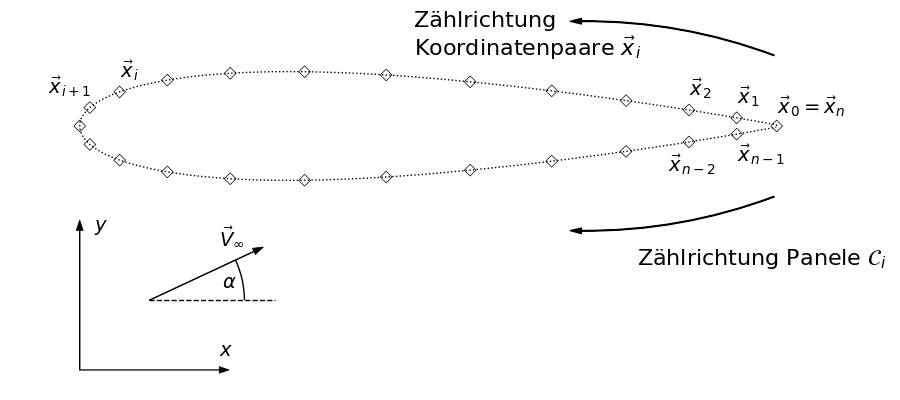
\includegraphics[scale=0.3]{figures/zaehlrichtung.png} \end{center}
\caption{Zur Definition der Zählrichtung der Panels sowie der Anströmgeschwindigkeit und deren Winkel}
\label{fig:zaehlrichtung}
\end{figure}
Das Hess-Smith-Panelverfahren ist ein Verfahren zur Berechnung von ebenen Potentialströmungen um geschlossene Körper mit Auftrieb. Ein kontinuierlicher zweidimensionaler Körper mit der Umfangkurve $\mathcal{C}$ wird dabei zunächst durch  $n + 1$ diskrete Datenpunkte $\vec x_i = (x_i, y_i)$ dargestellt. Die Zählrichtung dieser Punkte sei als im Uhrzeigersinn festgelegt (siehe Abb. \ref{fig:zaehlrichtung}). Für das Profil gilt somit die Periodizität $\vec x_n = \vec x_0$.\\
Die Kontur des Profils wird nun durch eine endliche Anzahl Verbindungsgeraden zwischen zwei benachbarten Punkten $\vec x_i, \vec x_{i+1}$, den Panelen $\mathcal{C}_i$ (Abb. \ref{fig:panel}) angenähert. Dabei wird jedes Panel durch die folgenden Parameter charakterisiert:
\begin{itemize}
\item Den Mittelpunkten auf beiden Achsen: 
\begin{equation}
X_i =  \frac{x_{n-i}+x_{n-i-1}}{2}, \; Y_i =  \frac{y_{n-i}+y_{n-i-1}}{2},
\end{equation}
\item seinem Neigungswinkel: 
\begin{equation}
\theta_i =  \left( \frac{y_{n-i-1} - y_{n-i}}{x_{n-i-1} - x_{n-i}} \right),
\end{equation}
\item und seiner Länge: 
\begin{equation}
l_i =  \sqrt{(x_{n-i-1} - x_{n-i})^2 + (y_{n-i-1} - y_{n-i})^2}.
\end{equation}
\end{itemize}


\begin{figure}
\begin{center} 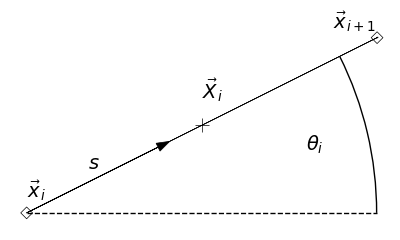
\includegraphics[scale=0.5]{figures/panel.png} \end{center}
\caption{Zur Definition eines Panels}
\label{fig:panel}
\end{figure}

Im Hess-Smith-Panelverfahren sei nun jedes dieser Panels mit einer vorerst unbestimmten, konstanten Quelldichte $q_i$ behaftet, welche an einem Punkt $\vec r_i =  \vec x - \hat x_i(s)$ zum Geschwindigkeitspotential den Beitrag
\begin{equation}
\label{eqn:potq}
\phi_i^{(q)} =  \frac{q_i}{2 \pi } \int_{\mathcal{C_i}} ds \ln r_i
\end{equation}
liefert. $s$ ist dabei die Koordinate der Bogenlänge, welche das gesamte Profil parametrisiert. \\
Ebenso liefert die Profilanströmung mit der konstanten Geschwindigkeit $V_{\infty}$ unter dem Winkel $\alpha $ ein Potential
\begin{equation}
\label{eqn:potv}
\phi_{\infty} =  V_{\infty} (\cos \alpha x + \sin \alpha y).
\end{equation}
Aus der Summe über alle Panelbeiträge aus (\ref{eqn:potq}) und (\ref{eqn:potv}) ergibt sich das Gesamtgeschwindigkeitspotential zu
\begin{equation}
\label{eqn:potnovortex}
\phi(\vec x) =  V_{\infty} (\cos \alpha x + \sin \alpha y) + \sum_{i=0}^{n-1} \phi_i^{(q)}.
\end{equation}
Daraus folgt für die Geschwindigkeit im Punkte $\vec x$ 
\begin{equation}
\vec v ( \vec x) =  \nabla  \phi (\vec x).
\end{equation}
Auf der Oberfläche des Profils muss die Strömung die Gleitbedingung erfüllen; damit lassen sich $n$ Gleichungen aufstellen, um diese Bedingung zu modellieren. Wir verlangen, dass die Normalkomponente des Geschwindigkeitsvektors,
\begin{equation}
v_j^{(n)} =  \vec v(\vec X_j) \cdot \vec n_j,
\end{equation}
verschwindet. Dabei ist $\vec n_j$ der Normalvektor auf das Panel $\mathcal{C}_j$.\\
Wir erhalten in 0. Ordnung ein System von $n$ Gleichungen
\begin{equation}
\label{eq:lgls1}
\sum_{j=0}^{n-1} M_{ij}^{(q)}q_j =  b_i,
\end{equation}
mit
\begin{equation}
M_{ij}^{(q)} = \frac{1}{q_j} \nabla \phi_j^{(q)} (\vec X) \cdot \vec n_i,
\end{equation}
\begin{equation}
b_i =  -V_{\infty} \left( \begin{matrix} \cos \alpha \\ \sin \alpha \end{matrix} \right) \cdot \vec n_i,
\end{equation}
aus dessen Lösung wir die Quellstärken $q_i$ für jedes Panel ermitteln können. \\
Damit kann nun der Tangentialkomponenten des Geschwindigkeitsvektors
\begin{equation}
\label{eqn:vt}
v_j^{(t)} =  \vec v(X_j) \cdot \frac{\vec x_{j+1}-\vec x_j}{|\vec x_{j+1}-\vec x_j|},
\end{equation}
bestimmt werden. \\
Aus der Bernoulli-Gleichung
\begin{equation}
p_{\infty} + \frac{1}{2} \rho V_{\infty}^2 =  p + \frac{1}{2} \rho v^2,
\end{equation}
definieren wir den Druckbeiwert als das Verhältnis zwischen der Druckdifferenze zwischen der Profilanströmung und dem dynamischen Druck 
\begin{equation}
c_p =  \frac{p-p_{\infty}}{\frac{1}{2} \rho V_{\infty}^2}.
\end{equation}
Daraus können wir den Druckbeiwert
\begin{equation}
c_{p_j} =  1 - \left( \frac{v_j^{(t)}}{V_{\infty},}\right)
\end{equation}
am Mittelpunkt des Panels $\mathcal{C}_j$ bestimmen.
\subsection{Berücksichtigung einer Wirbelbewegung}
Wollen wir den Auftrieb berücksichtigen, so reicht die reine Quellbelegung des Profils noch nicht aus. \\
Im Hess-Smith Verfahren nehmen wir für das gesamte Profil eine einzige konstante Wirbelbelegung $\gamma$ für alle Panels an. Damit wird das Potential (\ref{eqn:potnovortex}) erweitert um Beiträge
\begin{equation}
\phi_i^{(w)} =  \frac{\gamma}{2 \pi } \int ds \theta_i,
\end{equation}
zu
\begin{align}
\phi(\vec x) &=  V_{\infty} (\cos \alpha x + \sin \alpha y) + \sum_{i=0}^{n-1} \left( \phi_i^{(q)} + \phi_i^{(w)} \right) \nonumber \\
&= V_{\infty} (\cos \alpha x + \sin \alpha y) + \sum_{i=0}^{n-1} \int_{\mathcal{C}_i} \left( \frac{q_i}{2\pi } \ln r_i - \frac{\gamma}{2\pi } \theta_{i} \right) ds ´´
\end{align}
Die Gleitbedingung bleibt erhalten, allerdings muss das Gleichungssystem aber entsprechend dem hinzugekommenen Geschwindigkeitsbeitrag erweitert werden. Für die neue Unbekannte $\gamma$ fehlt also eine Gleichung. Diese ergibt sich aus der Kutta-Bedingung, welche besagt, dass es an der Hinterkante des Profils keine Umströmung gibt.\\
Zur Modellierung der Kutta-Bedingung wählen wir
\begin{equation}
v_0^{(t)} =  -v_n^{(t)}.
\end{equation} 
Daraus folgt, dass die Tangentialkomponenten des Geschwindigkeitsvektors in den Mittelpunkten der Panels, welche die Profilhinterkante bilden, vom Betrag gleich groß und gegenläufig gerichtet sein muss (siehe Abb. \ref{fig:kutta}). \\
Nach Lösung des erhaltenen linearen Gleichungssystems mit $q_n = \gamma$ können wir nun den Auftriebsbeiwert $c_a$ ermitteln. Dieser ergibt sich mit $t$, der Proftiltiefe und $l_i$, der Länge des Panels $\mathcal{C}_i$, approximiert in folgender Form:
\begin{equation}
c_a \approx \frac{2}{V_{\infty t}}\sum_{i=0}^{n-1} v_i^{(t)} l_i.
\end{equation}
\begin{figure}
\begin{center} 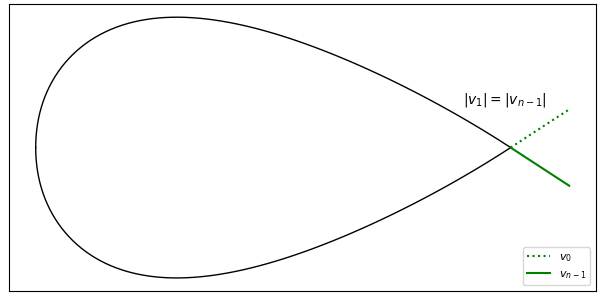
\includegraphics[scale=0.7]{figures/kutta.png} \end{center}
\caption{Zur Kutta-Bedingung am Beispiel eines NACA0012-Profils - am Punkt der Hinterkante sind die Tangentialgeschwindigkeiten genau entgegengerichtet}
\label{fig:kutta}
\end{figure}
Für eine analytische Berechnung des Auftriebsbeiwerts müssen wir nun noch die Systemmatrix bestimmen, welche das lineare Gleichungssystem (\eqref{eq:lgls1}) definiert. \cite{Hess:1966} \cite{Cebeci:1999} \cite{Alonso:2005}

\subsection{Berechnung der Systemmatrix}
\label{chap:systemmatrixtheory}
Die Systemmatrix zur Berechnung der Normalgeschwindigkeiten $v_i^{(n)}$ in den Panelmittelpunkten für eine stückweise konstante Quellenbewegung der Panels ergibt sich aus der Gleitbedingung. Wenden wir diese direkt auf \ref{eqn:potnovortex} an, muss ein kompliziertes Integral gelöst werden. Dieses kann theoretisch direkt mit Computermethoden gelöst werden, für den Berechnungsaufwand ist es allerdings gerade bei Profilen mit einer hohen Anzahl an Panels günstiger, dieses analytisch zu berechnen. \\
Für die Systemmatrix und ihre Parameter gelten:
\begin{equation}
M_{ij} = A_{ij}^{(n)}, \;\; i = 0, 1, \ldots , n-1; \;\; j = 0,1,\ldots , n-1.
\end{equation}
mit der Einflussmatrix der Quellbelegung
\begin{equation}
A_{ij}^{(n)} = -\sin {(\theta _i - \theta _j)} I_{ij} + \cos{(\theta _i - \theta _j)} J_{ij}
\end{equation}
sowie das geometrische Integral der Normalgeschwindigkeit
\begin{equation}
I_{ij} = 
     \begin{cases}
       \frac{1}{4\pi } \ln \left[ \frac{(l_j + 2 \xi_{ij})^2 + 4 \eta_{ij}^2}{(l_j -2 \xi _{ij})^2 + 4 \eta_{ij}^2} \right] &\quad i \neq j \\
       0 &\quad i = j \\
     \end{cases}
\end{equation}
und dem geometrischen Integral der Tangentialgeschindigkeit
\begin{equation}
J_{ij} = 
     \begin{cases}
       \frac{1}{2\pi } \arctan \left[ \frac{l_j - 2 \xi_{ij}}{2 \eta_{ij}} \right] + \frac{1}{2\pi } \arctan \left[ \frac{l_j + 2 \xi_{ij}}{2 \eta_{ij}} \right] &\quad i \neq j \\
       \frac{1}{2} &\quad i = j \\
     \end{cases}
\end{equation}
\begin{equation}
\xi_{ij} =  (X_i - X_j) \cos \theta _j + (Y_i - Y_j) \sin \theta _j
\end{equation}
\begin{equation}
\eta_{ij} =  -(X_i - X_j) \sin \theta _j + (Y_i - Y_j) \cos \theta _j
\end{equation}
Mit der Systemmatrix und den Inhomogenitäten $b_i$ können wir nun das lineare Gleichungssystem aus (\ref{eq:lgls1}) berechnen. \\
Für die Tangentialkomponente der Geschwindigkeit erhalten wir dann den Ausdruck
\begin{equation}
\label{eq:vtnovortex}
v_i^{(t)} =  \sum_{j=0}^{n-1} A_{ij}^{(t)} q_j + V_{\infty} \cos{(\alpha - \theta_i)},
\end{equation}
mit der Einflussmatrix der Wirbelbelegung
\begin{equation}
A_{ij}^{(t)} =  \cos{(\theta _i - \theta _j)} I_{ij} + \sin{(\theta _i - \theta _j)} J_{ij}.
\end{equation}
\\
Diese Systemmatrix berücksichtigt allerdings noch keine Wirbelbelegungen. Im Falle einer konstanten Wirbelbelegung $\gamma$ auf allen Panels erweitert sich die Dimension von $M_{ij}$ von $n \times n$ auf $(n+1) \times (n+1)$. Dadurch müssen folgende zusätzliche Elemente bestimmt werden:
\begin{equation}
M_{in} =  \sum_{j=0}^{n-1} A_{ij}^{(t)}, \;\; i=0,1,\ldots, n-1;
\end{equation}
\begin{equation}
M_{nj} =  A_{0j}^{(t)} + A_{n-1,j}^{(t)}, \;\; j =0,1,\ldots, n-1;
\end{equation}
\begin{equation}
M_{n,n} =  - \sum_{j=0}^{n-1} \left[ A_{0,j}^{(n)} + A_{n-1,j}^{(n)}\right];
\end{equation}
\begin{equation}
b_n =  -V_{\infty} [\cos{(\alpha -\theta 0)} + \cos{(\alpha -\theta _{n-1})}];
\end{equation}
Gleichung (\ref{eq:vtnovortex}) erweitert sich damit zu
\begin{equation}
v_i^{(t)} =  \sum_{j=0}^{n-1} A_{ij}^{(t)} q_j - \gamma \sum_{j=0}^{n-1}A_{i,j}^{(n)} + V_{\infty} \cos{(\alpha - \theta_i)}.
\end{equation}
\newpage
\chapter{Bericht der Arbeit}
Im Folgenden werden die wesentlichen Erkenntnisse der Arbeit präsentiert.
\section{Vorbereitung der Daten}
Die Daten der Profile wurden der UIUC Airfoil Data Site\footnote{\url{https://m-selig.ae.illinois.edu/ads/coord_database.html}} entnommen. Die Daten lagen dabei überwiegend im Selig- oder Lednicer-Format vor.\footnote{Eine Gegenüberstellung der beiden Formate ist in \nameref{appendix:a} zu finden.}
\\
Im Lednicer-Format wird in der ersten Zeile die Bezeichnung des Profils angegeben. In der zweiten Zeile wird die Anzahl der Koordinatenpaare der Ober- und Unterseite angegeben. Ab der dritten Zeile werden die Koordinaten der Panelenden $(x_i,y_i)$ von $x=0$ bis $x=1$ für die Oberseite des Profils angegeben. Danach folgt eine Leerzeile. Danach werden die Koordinaten der Panelenden $(x_i,y_i)$ von $x=0$ bis $x=1$ für die Unterseite des Profils angegeben.
\\
Im Selig-Format wird in der ersten Zeile die Bezeichnung des Profils angegeben. Ab der zweiten Zeile werden die Koordinaten der Panelenden $(x_i,y_i)$ im Gegenuhrzeigersinn, beginnend bei $x=1$ angegeben.
\\\\
Es wurde eine Routine geschrieben, welche Daten im Lednicer-Format in das Selig-Format überführt. Dies wurde bewerkstelligt, indem die Koordinatenpaare der Oberseite invertiert wurden. Anschließend wurden aus den Daten die Header-Zeilen entfernt. \\
Unter Verwendung der Methode .write\_file() wurde für sämtliche Profile eine .csv-Datei mit den Werten $X_i, Y_i, \theta _i, l_i$ pro Panel erstellt (eine Beispieldatei ist in \nameref{appendix:a} gezeigt. Ebenso wurde für jedes sih in der UIUC-Datenbank befindliche Trägerprofil ein Graph erzeugt, welcher zum einen die Geometrie des Profils, sowie auch die Neigungswinkel und Längen der einzelnen Panels darstellt. Zur einfacheren Betrachtung sind die Graphen der Neigungswinkel und Panellängen in die beiden Seiten des Profils aufgeteilt. 
\\Ein solcher Graph ist in Abbildung \ref{fig:naca0012} an einem NACA-0012-Profil gezeigt. Die Symmetrie des Profils spiegelt sich in der gewählten Darstellung der Neigungswinkel und Panellängen gut wieder.

\begin{figure}
\begin{center}
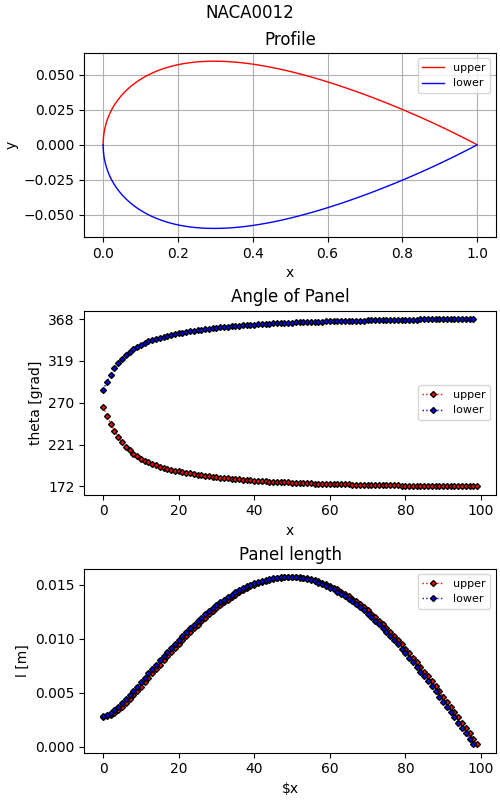
\includegraphics[scale=1]{figures/NACA0012.png} 
\caption{NACA-0012-Profil}
\label{fig:naca0012}
\end{center}
\end{figure}

\begin{table}
\label{tab:1}
\centering{
\begin{tabular}{cccc}
%\toprule
$X_i$ & $Y_i$         & $\theta_i$ & $l_i$ \\
%\midrule
0.8 & -0.35 & 67.5 & 0.77 \\
0.35 & -0.85 & 22.5 & 0.77 \\
-0.35 & -0.85 & 337.5 & 0.77 \\
-0.85 & -0.35 & 292.5 & 0.77 \\
-0.85 & 0.35 & 247.5 & 0.77 \\
-0.35 & 0.85 & 202.5 & 0.77 \\
0.35 & 0.85 & 157.5 & 0.77 \\
0.85 & 0.35 & 112.5 & 0.77

%\bottomrule
\end{tabular}
}
\end{table}

\begin{figure}[!h]
\begin{center}
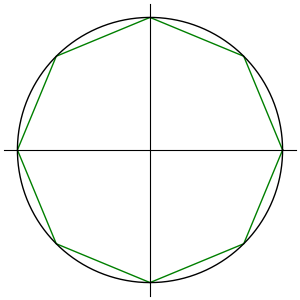
\includegraphics[scale=0.7]{figures/cylinderascircle.png} 
\caption{Achtseitiger Cylinder als Approximation eines Kreiszylinders sowie zugehörige Panelparameter}
\label{fig:cylinder8}
\end{center}
\end{figure}
\section{Untersuchungen am  Kreiszylinder}

Als nächstes wurden Untersuchung an Kreiszylindern vorgenommen, da bei diesen die Aufteilung in Panele relativ leicht zu implementieren ist. Zur Generierung eines Kreiszylinders mit $n$ gleich großen Seiten wurde die Funktion make\_cylinder(r, n) verwendet (siehe \nameref{appendix:c}).
\subsection{Achtseitiger Kreiszylinder}
\subsubsection{Berechnung der Systemmatrix}
Für den in \ref{fig:cylinder8} gezeigten Kreisylinder wurde die Systemmatrix zu folgenden Werten berechnet:
\begin{align*}
M_{i,j} = 
\begin{pmatrix}
0.5&0.056&0.064&0.065&0.065&0.065&0.064&0.056 \\
0.056&0.5&0.056&0.064&0.065&0.065&0.065&0.064\\
0.064&0.056&0.5&0.056&0.064&0.065&0.065&0.065\\
0.065&0.064&0.056&0.5&0.056&0.064&0.065&0.065\\
0.065&0.065&0.064&0.056&0.5&0.056&0.064&0.065\\
0.065&0.065&0.065&0.064&0.056&0.5&0.056&0.064\\
0.064&0.065&0.065&0.065&0.064&0.056&0.5&0.056\\
0.056&0.064&0.065&0.065&0.065&0.064&0.056&0.5
\end{pmatrix}
\end{align*}
\subsubsection{Lösung des wirbellosen Gleichungssystems}
\subsection{Untersuchungen an variierenden Kreiszylindern}
\subsubsection{Variation der Panelanzahl}
\subsubsection{Rotation des Zylinders}
\section{Untersuchungen an ausgewählten Profilen}
\subsection{NACA0012-Profil}
\subsection{Joukowsky 12\%-Profil}
\subsection{Fehlerabschätzung des Hess-Smith-Verfahrens}




\newpage
%\chapter{Mathematik}
\bigskip
Issue with mapsto : ${\mathcal F} : \boldsymbol{\eta} \in {\mathbb{R}}^{np}\ \mapsto {\mathcal F}\left(\boldsymbol{\eta} \right)\in \mathbb{R}$

\bigskip
Issue with sqrt : $\sqrt{X}$

\bigskip
Issue with parenthesis : $X \geqslant \left(\frac{1}{2}\right)^2$

\bigskip
Issue with sum : $\sum_{n=0}^\infty X^n$
\newpage

\cleardoublepage
\pagenumbering{roman} \setcounter{page}{1}
\printbibliography
%\chapter*{Danksagung}

Ein großer Dank für dieses Werk geht an die Community des Versionskontrollsystems GIT und dessen Erfinder Linus Torvalds. Ohne GIT wäre die Entwicklung, selbst einer so einfachen \LaTeX Vorlage sehr viel aufwändiger gewesen. Ich möchte auf diesem Weg auch allen die mit dieser Vorlage arbeiten empfehlen GIT zu verwenden. Es wird euer Leben sehr viel einfacher machen und ist noch dazu gratis und quelloffen inklusive Dokumentation und Buch verfügbar.
\begin{center}
GIT: \url{http://git-scm.com/} \\
Buch: \url{http://git-scm.com/book}
\end{center}
\newpage
\newpage
\appendix
\appendix

\addsec{Anhang A: Lednicer- und Selig-Format}
\label{appendix:a}

Es folgt eine Gegenüberstellung des Selig-Formats (links) mit dem Lednicer-Format (rechts) am Beispiel des NACA M13-Profils.

\begin{minipage}{0.45\textwidth}
\verbatiminput{dataformats/m13_selig.DAT}
\end{minipage}
    \hfill
\begin{minipage}{0.45\textwidth}
\verbatiminput{dataformats/m13_lednicer.DAT}
\end{minipage}

\newpage
\addsec{Anhang B: Beispielausgabe der Methode .write\_panels()}
\label{appendix:b}
Hier ist die Ausgabe der ersten 30 Zeilen der AirfoilProfile-Methode .write\_panels() gezeigt, am Beispiel des NASA: HSNLF(1)-0213 Profils.

\verbatiminput{writtenvals/hsnlf213_vals.csv}

\newpage
\addsec{Anhang C: Codeausschnitte}
\label{appendix:c}
Hier sind ausgewählte Codeausschnitte gezeigt, welche zur Lösung der Problemstellungen geschrieben wurden.
\subsubsection{Die Klasse Panel}
Die Klasse Panel modelliert die Panels $\mathcal{C}_i$ eines gegebenen Profils. Gespeichert werden neben den charakteristischen Parametern $X_i, Y_i, \theta _i, l_i$ auch der Normalwinkel des Panels $\delta_i$, welcher aus dem Profil herauszeigt. Ebenso wird die Panelposition als Ober- oder Unterseite bestimmt (für einige besondere Profile ist auch ein Wert "vertical" für komplett senkrechte Panele möglich). Ebenso gespeichert wird die Quellbelegung $q_i$, die Tangentialgeschwindigkeit $v_i^{(t)}$ unter gegebenen Anströmwinkel $\alpha $ und -geschwindigkeit $V_{\infty}$, und der resultierende Druckbeiwert $c_{p_i}$.
\begin{lstlisting}[language=Python]
class Panel:

    def __init__(self, xa, ya, xb, yb):
        self.xa, self.ya = xa, ya
        self.xb, self.yb = xb, yb

        self.xm = (xa + xb) / 2
        self.ym = (ya + yb) / 2
        self.length = np.sqrt((xb - xa) ** 2 + (yb - ya) ** 2)
        self.theta = np.arctan2(yb - ya, xb - xa)

        self.q = None
        self.vt = None
        self.cp = None
\end{lstlisting}

\subsubsection{Die Klasse AirfoilProfile}
Die Klasse AirfoilProfile modelliert ein gegebenes Profil. Sie speichert neben wählbaren Namen und der ihr zugewiesenen Panele auch die Profiltiefe $t$ und sämtliche Systemparameter $\xi_{ij}, \; \eta_{ij}, \; I_{ij}, \; J_{ij}, \; A_{ij}^{(n)}, \;A_{ij}^{(t)}, \;M_{ij}$. \\
Durch einen Aufruf der Methode .solve(V, a) mit gegebenen $\alpha $ und $V_{\infty}$ werden für alle zugeordneten Panele die Quellstärken, Tangentialgeschwindigkeiten und Druckbeiwerte berechnet (und in den jeweiligen Klassenvariablen abgespeichert). Dabei wird ebenfalls die Genauigkeit der Approximation $\sum q_i l_i$ berechnet. Die Methode kann mit dem Schlüsselwortargument vortex=True aufgerufen werden, wodurch ebenfalls der Auftriebsbeiwert $c_a$, sowie die Wirbelbewegung $\gamma$ \\ berechnet werden.
Die Methode .write\_panels() erzeugt eine .csv-Datei, welche für jedes Panel die Werte $X_i, Y_i \theta_i, l_i$ in eine Zeile schreibt (siehe \nameref{appendix:a}). \\
Die Methode .compute\_free\_vt(x, y, V, a) ermöglicht die Berechnung der Tangentialgeschwindigkeiten an jedem Punkt $(x_i, y_i)$ des Profils. Diese werden als Tupel von der Methode zurückgegeben.
\begin{lstlisting}[language=Python]
class AirfoilProfile:
    def __init__(self, panels, name=None, vortex=True):
        self.panels = panels
        self.name = name
        self.x = [panel.xa for panel in self.panels]
        self.y = [panel.ya for panel in self.panels]
        self.len = len(self.panels)
        self.vortex = vortex
        self.shape = Polygon([(a,b) for a,b in zip(self.x, self.y)])

        self.U = sum([panel.length for panel in self.panels])
        self.t = abs(max(self.x) - min(self.x))

        self.xi = self.__xi()
        self.eta = self.__eta()
        self.I = self.__i()
        self.J = self.__j()
        self.An = self.__an()
        self.At = self.__at()
        self.M = self.__m()

        self.solve_state = None
        self.ca = None
        self.accuracy = None
        self.gamma = None

    def write_panels(self, filename, n=2):
        header = ["X_i", "Y_i", "theta_i", "l_i"]
        with open(filename, "w+", encoding='UTF8',newline="") as file:
            writer = csv.writer(file)
            writer.writerow(header)
            for panel in self.panels:
                writer.writerow([round(panel.xm,n), round(panel.ym,n), round(panel.theta*180/np.pi,n), round(panel.length,n)])

    def __xi(self, x=None, y=None):
        panels = self.panels
        n_panels = len(panels)
        if x is not None and y is not None:
            n = 1
        else:
            n = len(panels)
        Xi = np.empty((n, n_panels), dtype=float)
        for i in range(n):
            for j in range(n_panels):
                if x is not None and y is not None:
                    i_xm, i_ym = x, y
                else:
                    i_xm, i_ym = panels[i].xm, panels[i].ym
                pj = panels[j]
                Xi[i][j] = (i_xm - pj.xm) * np.cos(pj.theta) + (i_ym - pj.ym) * np.sin(pj.theta)
        return Xi

    def __eta(self, x=None, y=None):
        panels = self.panels
        n_panels = len(panels)
        if x is not None and y is not None:
            n = 1
        else:
            n = len(panels)
        Eta = np.empty((n, n_panels), dtype=float)
        for i in range(n):
            for j in range(n_panels):
                if x is not None and y is not None:
                    i_xm, i_ym = x, y
                else:
                    i_xm, i_ym = panels[i].xm, panels[i].ym
                pj = panels[j]
                Eta[i][j] = - (i_xm - pj.xm) * np.sin(pj.theta) + (i_ym - pj.ym) * np.cos(pj.theta)
        return Eta

    def __i(self, Xi=None, Eta=None):
        panels = self.panels
        if Xi is None and Eta is None:
            Xi = self.xi
            Eta = self.eta
        n_panels = len(panels)
        n = Xi.shape[0]
        II = np.empty((n, n_panels), dtype=float)
        for i in range(n):
            for j in range(n_panels):
                pj = panels[j]
                if i == j and n > 1:
                    II[i][j] = 0
                else:
                    II[i][j] = (1 / (4 * np.pi)) * np.log(((pj.length + 2 * Xi[i][j]) ** 2 + 4 * (Eta[i][j] ** 2)) / ((pj.length - 2 * Xi[i][j]) ** 2 + 4 * (Eta[i][j] ** 2)))
        return II

    def __j(self, Xi=None, Eta=None):
        panels = self.panels
        if Xi is None and Eta is None:
            Xi = self.xi
            Eta = self.eta
        n_panels = len(panels)
        n = Xi.shape[0]
        JJ = np.empty((n, n_panels), dtype=float)
        for i in range(n):
            for j in range(n_panels):
                pj = panels[j]
                if i == j and n > 1:
                    JJ[i][j] = 0.5
                else:
                    JJ[i][j] = (1 / (2 * np.pi)) * np.arctan((pj.length - 2 * Xi[i][j])/ (2 * Eta[i][j])) + (1 / (2 * np.pi)) * np.arctan((pj.length + 2 * Xi[i][j])/ (2 * Eta[i][j]))
        return JJ

    def __an(self, II=None, JJ=None):
        panels = self.panels
        if II is None and JJ is None:
            II = self.I
            JJ = self.J
        n_panels = len(panels)
        n = II.shape[0]
        if n == 1:
            i_theta = 0
        AN = np.empty((n, n_panels), dtype=float)
        for i in range(n):
            for j in range(n_panels):
                if n > 1:
                    i_theta = panels[i].theta
                pj = panels[j]
                AN[i][j] = - np.sin(i_theta - pj.theta) * II[i][j] + np.cos(i_theta - pj.theta) * JJ[i][j]
        return AN

    def __at(self, II=None, JJ=None):
        panels = self.panels
        if II is None and JJ is None:
            II = self.I
            JJ = self.J
        n_panels = len(panels)
        n = II.shape[0]
        if n == 1:
            i_theta = 0
        AT = np.empty((n, n_panels), dtype=float)
        for i in range(n):
            for j in range(n_panels):
                if n > 1:
                    i_theta = panels[i].theta
                pj = panels[j]
                AT[i][j] = np.cos(i_theta - pj.theta) * II[i][j] + np.sin(i_theta - pj.theta) * JJ[i][j]
        return AT

    def __m(self):
        panels = self.panels
        AN = self.An
        AT = self.At
        vortex = self.vortex
        n = len(panels)
        if vortex:
            MM = np.empty((n + 1, n + 1), dtype=float)
        else:
            MM = np.empty((n, n), dtype=float)
        if vortex:
            MM[:-1, :-1] = AN
            MM[:-1, -1] = np.sum(AT, axis=1)

            r = np.empty(n + 1, dtype=float)
            r[:-1] = AT[0, :] + AT[n - 1, :]
            r[-1] = -np.sum(AN[0, :] + AN[n - 1, :])
            MM[-1, :] = r
        else:
            MM = AN
        return MM

    def solve(self, V=1, a=5):
        a = np.radians(a)
        b = self.__b(V, a)

        self.__q(b)  # setzt auch self.gamma
        self.__vt(V, a)
        self.__cp(V)
        self.__ca(V)
        self.__accuracy()
        self.solve_state = (V,a)

    def compute_free_vt(self, x, y, V=1, a=5):
        if (V,a) != self.solve_state:
            self.solve(V=V, a=a)
        a = np.radians(a)
        point = Point(x,y)
        if point.within(self.shape) or self.shape.touches(point):
            vtx = np.nan
            vty = np.nan
        else:
            xi = self.__xi(x=x, y=y)
            eta = self.__eta(x=x, y=y)
            I = self.__i(Xi=xi, Eta=eta)
            J = self.__j(Xi=xi, Eta=eta)
            An = self.__an(II=I, JJ=J)
            At = self.__at(II=I, JJ=J)

            vtx = sum([At[0][j] * self.panels[j].q for j in range(self.len)]) - self.gamma * sum(
                [An[0][j] for j in range(self.len)]) + V * np.cos(a)

            vty= sum([An[0][j] * self.panels[j].q for j in range(self.len)]) + self.gamma * sum(
                [At[0][j] for j in range(self.len)]) + V * np.sin(a)

        return vtx, vty

    def __b(self, V, a):
        panels = self.panels
        vortex = self.vortex
        n = len(panels)
        if vortex:
            B = np.empty(n + 1, dtype=float)
        else:
            B = np.empty(n, dtype=float)
        for i in range(n):
            pi = panels[i]
            B[i] = -V * np.sin(a - pi.theta)
        if vortex:
            B[-1] = -V * (np.cos(a - panels[0].theta) + np.cos(a - panels[-1].theta))
        return B

    def __q(self, B):
        panels = self.panels
        qs = np.linalg.solve(self.M, B)

        for i, panel in enumerate(panels):
            panel.q = qs[i]
        if self.vortex:
            self.gamma = qs[-1]

    def __vt(self, V, a):
        panels = self.panels
        AN = self.An
        AT = self.At
        n = len(panels)
        if self.vortex:
            VT = np.empty(n, dtype=float)
            for i in range(n):
                VT[i] = sum([AT[i][j] * panels[j].q for j in range(n)]) \
                        - self.gamma * sum([AN[i][j] for j in range(n)]) \
                        + V * np.cos(a - panels[i].theta)
        else:
            VT = np.empty(n, dtype=float)
            for i in range(n):
                VT[i] = sum([AT[i][j] * panels[j].q for j in range(n)]) \
                        + V * np.cos(a - panels[i].theta)

        for i, panel in enumerate(panels):
            panel.vt = VT[i]

    def __cp(self, V):
        for panel in self.panels:
            panel.cp = 1 - (panel.vt / V) ** 2

    def __ca(self, V):
        self.ca = 2 / (V * self.t) * sum([panel.vt * panel.length for panel in self.panels])

    def __accuracy(self):
        self.accuracy = sum([panel.q * panel.length for panel in self.panels])


\end{lstlisting}

\subsubsection{make\_cylinder(r,n)}
Diese Funktion wurde verwendet, um die $x$- und $y$-Koordinaten eines Kreiszylinder mit Radius $r$ und $n$ gleich langen Panels zu generieren. Es wurde dabei besonderes Augenmerk darauf gelegt, dass es an den Endpunkten durch Rundungsfehler nicht zu einem disjunkten Körper kommt.
\begin{lstlisting}
def cylinder(r=1, n=8):
    a = np.linspace(0, 360, num=n+1, endpoint=True) / 180 * np.pi

    x = r * np.cos(a)
    y = r * np.sin(a)
    if abs(x[0] - x[-1]) <= 10 ** (-15):
        x[-1] = x[0]
    if abs(y[0] - y[-1]) <= 10 ** (-15):
        y[-1] = y[0]

    return x, y
\end{lstlisting}

\subsubsection{make\_panels(x,y, reverse=False)}
\begin{lstlisting}
    if type(x) is not np.ndarray:
        x = np.array(x)
    if type(y) is not np.ndarray:
        y = np.array(y)
    if (x[0], y[0]) != (x[-1], y[-1]):
        x = np.append(x, x[0])
        y = np.append(y, y[0])
    if reverse:
        x = np.flipud(x)
        y = np.flipud(y)
    n = len(x) - 1
    panels = np.array([Panel(x[i], y[i], x[i + 1], y[i + 1]) for i in range(n)])
    return panels
\end{lstlisting}

\subsubsection{parsecoords(filename)}
\begin{lstlisting}
    x, y = np.loadtxt(filename, dtype=float, unpack=True)
    return x, y
\end{lstlisting}

\subsubsection{Joukowsky-Profil-Generator}

\begin{lstlisting}
def joukowski_transfrom(zeta):
    z = zeta + 1 / zeta
    return z
def make_joukowski(mux=0.2, muy=0.1, N=100):
    center = -mux + muy * 1j 
    R = np.sqrt((1 + mux) ** 2 + muy ** 2)

    theta = np.linspace(0, 2 * np.pi, N)
    Xc = np.real(center) + R * np.cos(theta)
    Yc = np.imag(center) + R * np.sin(theta)

    p = joukowski_transfrom(Xc + Yc * 1j)
    Xp, Yp = np.real(p), np.imag(p)
    return Xp, Yp, R, muy
\end{lstlisting}

\subsubsection{Kármán-Trefftz-Profil-Generator}

\begin{lstlisting}
def karman_trefftz_transform(zeta, n):
    z = n * ((zeta + 1) ** n + (zeta - 1) ** n) / ((zeta + 1) ** n - (zeta - 1) ** n)
    return z
def make_karman_trefftz(mux=0.2, muy=0.1, n=1.9, N=100):
    center = -mux + muy * 1j
    R = np.sqrt((1 + mux) ** 2 + muy ** 2) 

    theta = np.linspace(0, 2 * np.pi, N)
    Xc = np.real(center) + R * np.cos(theta)
    Yc = np.imag(center) + R * np.sin(theta)
    tx = np.real(center)
    ty = np.imag(center)

    p = karman_trefftz_transform(Xc + Yc * 1j, n)
    Xp, Yp = np.real(p), np.imag(p)
    return Xp, Yp, R, muy
\end{lstlisting}




\end{document}